\documentclass[12pt]{article}
\usepackage{fullpage}
\usepackage{mathpazo}
\renewcommand{\baselinestretch}{1.2}
\usepackage{enumerate}
\usepackage[parfill]{parskip}
\usepackage{amsfonts}
\usepackage{graphicx}
\usepackage{titlesec}
\usepackage{enumitem}
\usepackage{hyperref}
\newcommand{\sectionbreak}{\clearpage}
\graphicspath{ {./images} }


\begin{document}
\begin{titlepage}
  \begin{center}
      \vspace*{1cm}

      
\includegraphics[width=14cm]{unsw-logo.png}

      \Huge
      \textbf{COMP9900 Information Technology Retrospective A}

      \vspace{0.5cm}
      \LARGE
      Car Space Renting System
           
      \vspace{1.5cm}
      \large
      [Scrum Master]
      \textbf{Huichuan Xu} z5212102@ad.unsw.edu.au z5212102 Backend\\
      \textbf{Fang Liu} z5235533@ad.unsw.edu.au z5235533 Backend\\
      \textbf{Jie Yuan} z5315183@ad.unsw.edu.au z5315183 Backend\\
      \textbf{Zeyang Zhang} zeyang.zhang@student.unsw.edu.au z5273456 Frontend\\
      \textbf{Qinjian Zheng} qinjian.zheng@student.unsw.edu.au z5325742 Frontend\\

      \vfill
      \Large
      Group Name: NoBUG\\
      Date: June 29, 2022
           
  \end{center}
\end{titlepage}
\tableofcontents
\section{Background}
  \subsection{Problem Review}

  While finding a temporary parking space is easy, it is hard to find a long-term parking space. You may have one at home, but what about when you drive to work? You may need to go to different advertisement websites to look for your answer. The same can be said for those that have parking space to rent, they need to post their ads on different platforms for a maximum exposure rate. So why not just have a designated platform for those who want to rent a parking space and those who have one or more to rent. That is why we want to build this car space renting system. This will become the one-stop solution for your next long-term parking space.

  With the increase of urban population and vehicle quantity, the problem of urban parking becomes more and more prominent. Especially in CBD areas of big cities, people may have to spend a long time looking for a suitable parking space and have to pay high parking fees. In addition, after the outbreak of COVID-19, due to people's panic over the epidemic, social distancing requirements, and restrictions on public transport rules, the utilization rate of public transport dropped significantly. Taking Australia as an example, the passenger capacity of public transport dropped to about 30\% of the original\cite{covid-travel}. As a result, private cars have become more dominant and parking spaces are in short supply.
  
  However, the problem of parking space shortage in urban areas is not caused by the lack of parking space. In fact, while the public parking spaces are full, many private parking spaces are completely empty. For example, when car owners drive their cars to work, their parking space will be free throughout the working hours. They can rent out these parking spaces to people in need and also earn some extra income.
  
  Therefore, this project aims to develop a parking space renting website, so people can rent/lease parking spaces based on their needs.
  
  \subsection{Existing Systems Case Study}

  Since similar systems and platforms exist, we will use them as a case study to determine what functionalities we should have and if they are lacking any functionality so that we can improve on them.

  We investigate three systems: Parkhound, Share with Oscar, and Parking Made Easy. All of which are web-site based while some of them also provide mobile applications. For the scope of this project, we think the website is enough for most users as it can be used both on desktop and mobile devices.
  
  Two of them do not require login or sign up to view parking listings. This is a feature for convenience and we think it can attract more casual looking-around potential users.
  
  In terms of basic layout, they also share some similarities. They tend to put the listings on the left side and have a map on the right side indicating where these listings are. It is clear and efficient for users to navigate to the ones they want.
  
  They are designed based on user roles. Different users should see different layouts and interact with the application differently. For example, a customer should be able to see a list of car spaces for renting while a provider should see a list of the car spaces he/she provides. Therefore, in our design, we need to customize the pages based on user roles.
  
  After investigating these systems, we think they lack certain functionalities that we can improve. Specifically, we can make recommendations to customers based on their previous renting histories, and customers can have their own wishlist listing their preferences. Whenever there is a car space that matches the preferences, customers will be notified via website notification or email. 
  
  \begin{center}
  \begin{table}[h!]
  \begin{tabular}{ |c|c|c|c| } 
  \hline
    & Parkhound & Share with Oscar & Parking Made Easy\\
  \hline
  Search without Login & Yes & Yes & No\\
  \hline
  Provides Map & Yes & Yes & Yes\\
  \hline
  Provides Mobile Application & Yes & Yes & No\\
  \hline
  Different User Roles & Yes & Yes & Yes\\
  \hline
  UI Design & Good & Good & Fair\\
  \hline
  Recommendations & Fixed & Fixed & No\\
  \hline
  Subscription & No & No & No\\
  \hline
  \end{tabular}
  \caption{Compare different systems}
  \label{table:1}
  \end{table}
  \end{center}

\section{User stories and sprints}

\subsection{User roles}

\begin{enumerate}
  \item Provider
  \item Customer
  \item Admin
\end{enumerate}

\subsection{Objectives/Functionalities \& User Stories}

\subsubsection{User Authorization}

Users of all types can sign up, login and logout the system.

\begin{enumerate}
  \item As a customer, I want to set up an account on the website and register my personal and vehicle details so that I can rent car spaces on the website.
  \item As a provider, I want to set up an account on the website so that I can use the website's service and post my car space on it.
\end{enumerate}

\subsubsection{User Profile}

Customers and providers can manage their own accounts and update personal information.

\begin{enumerate}[resume]
  \item As a customer, I want to update my personal information including contact information, billing address, vehicle information, etc. so that I can keep my information up-to-date.
  \item As a provider, I want to update my personal information including bank account details so that I can keep my information up-to-date.
  \item As a customer, I want to have a dashboard so that I can manage all my settings and rental history.
  \item As a provider, I want to have a dashboard so that I can check and manage all my listings of car spaces.
\end{enumerate}

\subsubsection{Admin CRUD}

Admin can create/read/update/delete (CRUD) all data of customers and providers, including account information, vehicle details, car space listings and rental histories.

\begin{enumerate}[resume]
  \item As an admin, I want to have a dashboard so that I can manage all users and listings.
\end{enumerate}

\subsubsection{Provider CRUD}

Providers can CRUD car space listings including registering new car spaces, checking all registered car spaces, updating existing car space information, and removing car spaces from the website.

\begin{enumerate}[resume]
  \item As a provider, I want to have a dashboard so that I can check and manage all my listings of car spaces.
  \item As a provider, I want to register a new car space including the cost per hour/day, and availability so that I can make my car space available for renting.
  \item As a provider, I want to update registered car space details so that I can match the registered car space on the website with my situation.
  \item As a provider, I want to remove a registered car space when I don't want to rent it anymore so that I don't get bookings for car spaces I don't intend to rent out.
\end{enumerate}

\subsubsection{Customer CRUD}

Customers can CRUD car space bookings including booking new car space, checking all bookings made, updating the current booking, and canceling the current booking.

\begin{enumerate}[resume]
  \item As a customer, I want to browse the list of all car spaces without logging in so that it is more convenient for me.
  \item As a customer, I want to see the list of all car spaces on a map so that I can better understand where they are.
  \item As a customer, I want to have a filter on listings so that I can find the one I need more efficiently.
  \item As a customer, I want to see details about the car space when I make a booking so that I know all the information about the car space.
  \item As a customer, I want to book a car space with a specified duration so that I can have a car space ready when I need it.
  \item As a customer, I want to know where I can park easily so that I will not damage other people's vehicles when my driving skill is not good.
  \item As a customer, I want to know the charging equipment around the parking space so that I can charge my electronic car easily.
  \item As a customer, I prefer to keep my search history on my homepage so that it is easy to reference.
  \item As a customer, I want to cancel a booking when I no longer need it so that I don't have to pay for it.
  \item As a customer, I want to update the booking information so that it can better suit my needs.
\end{enumerate}

\subsubsection{Payment}

System should have a payment process.

\begin{enumerate}[resume]
  \item As a customer, I want to receive bills both on the website when I book a car space and through email so that I can have a record of the car space I book.
  \item As a customer, I want to pay bills online so that I do not have to go to the bank.
  \item As a provider, I want to receive payments to my registered bank account details from the website so that I can get paid for my car space.
  \item As a provider, I want to rent my car space to other customers when the customer who books the car space does not complete the booking process in a certain amount of time so that I do not lose potential customers.
  
\end{enumerate}

\subsubsection{Ratings and Reviews}

Customers can rate and review the car space afterwards.

\begin{enumerate}[resume]
  \item As a customer, I want to rate the car space after parking and write a review about it so that I can share my opinions with other customers and give feedback to the provider.
  \item As a provider, I want to review the ratings and reviews of my car spaces so that I can better understand the customers' needs.
\end{enumerate}

\subsubsection{Subscription \textit{(novel)}}

System should enable customers and providers to subscribe to the website.

\begin{enumerate}[resume]
  \item As a customer, I want to set a wish list indicating my preference for future rentals and receive an email when there is one satisfying my requirement so that I do not need to keep an eye on the website all the time.
  \item As a provider, I want to know which customer is the first time using this system so that I can give him/her a discount to attract him/her to use it again.
  \item As a provider, I want to know which parking space has a problem in time so that I can ask some staff to solve the problem.
  \item As a provider, I want to know which parking space is the least efficient so that I can remove it from the system.
  \item As a provider, I want to receive notifications when there is a new cheaper car space near my offer so I can adjust the price and stay competitive.
\end{enumerate}

\subsubsection{Recommendation \textit{(novel)}}

System can recommend customers based on their preferences. Instead of one on-off switch, customers have several setting choices to choose from.

\begin{enumerate}[resume]
  \item As a customer, I want to receive recommendations based on my rental history so that I do not need to search every time.
  \item As a customer, I want to be recommended for the nearest parking location when I first search so that I can save the trouble of searching.
  \item As a customer, I want to dislike car spaces that I will not be renting so that I can focus more on car spaces I want.
\end{enumerate}

\subsubsection{Accessibility}

System should be user-friendly and suitable to use on devices of various sizes.

\begin{enumerate}[resume]
  \item As a website user, I want the website to be suitable for viewing on both desktop and mobile devices so that I can use it with ease anywhere.
  \item As a website user, I want the website to adjust the color theme automatically based on my system setting so that I can use it more comfortably.
\end{enumerate}

\subsection{Novel Features}

In order to improve the user experience on our application and after reviewing several existing applications on the market, we propose "Subscription" and "Recommendation" as our novel features for the application.

"Subscription" provides customization for users, which guarantee that users can have their own ways of using the application. While "Recommendation" harnesses the power of data analysis and smart algorithms to better serve the users. They work together to enhance the usability of the application.

\subsection{Backlog and Sprint 1}
  \begin{figure}[htp]
    \centering
    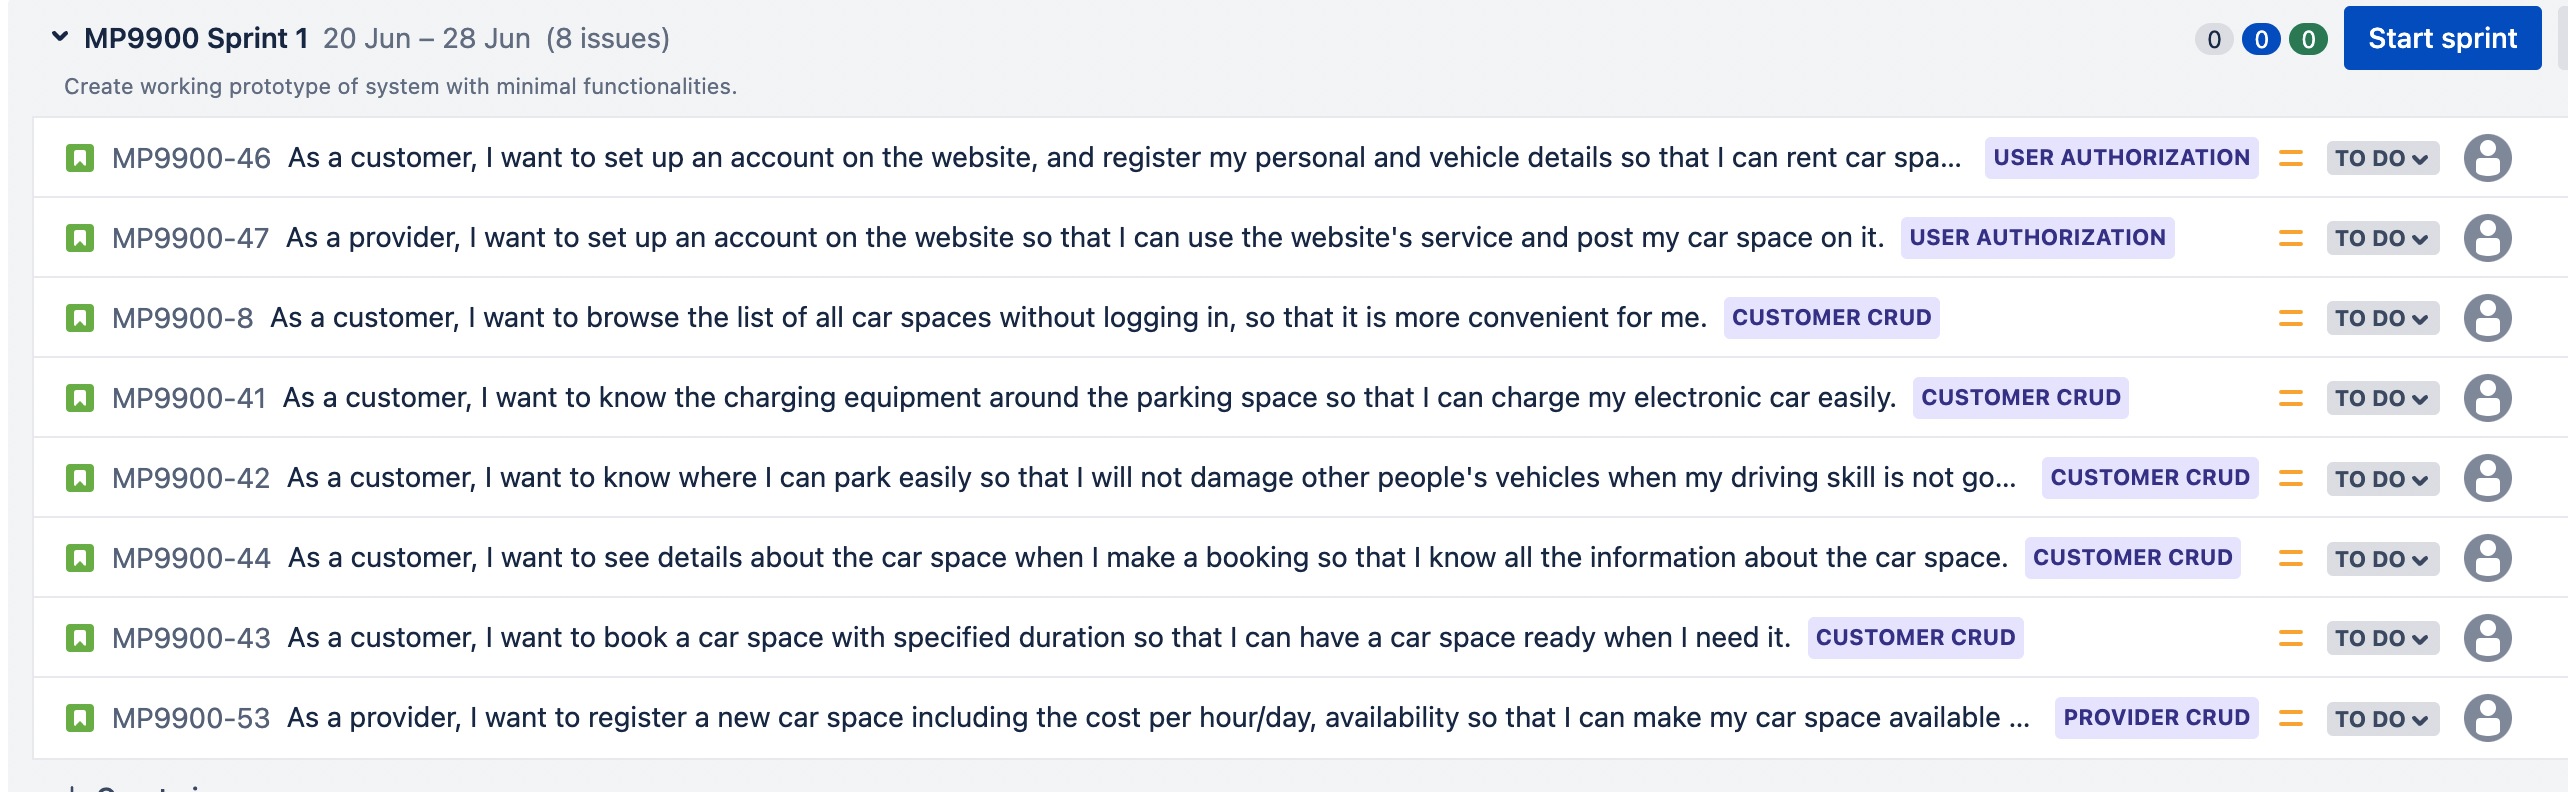
\includegraphics[width=\textwidth]{sprint1.png}
  \caption{Sprint 1 with user stories from Jira}
  
  \end{figure}

  \begin{figure}[htp]
    \centering
    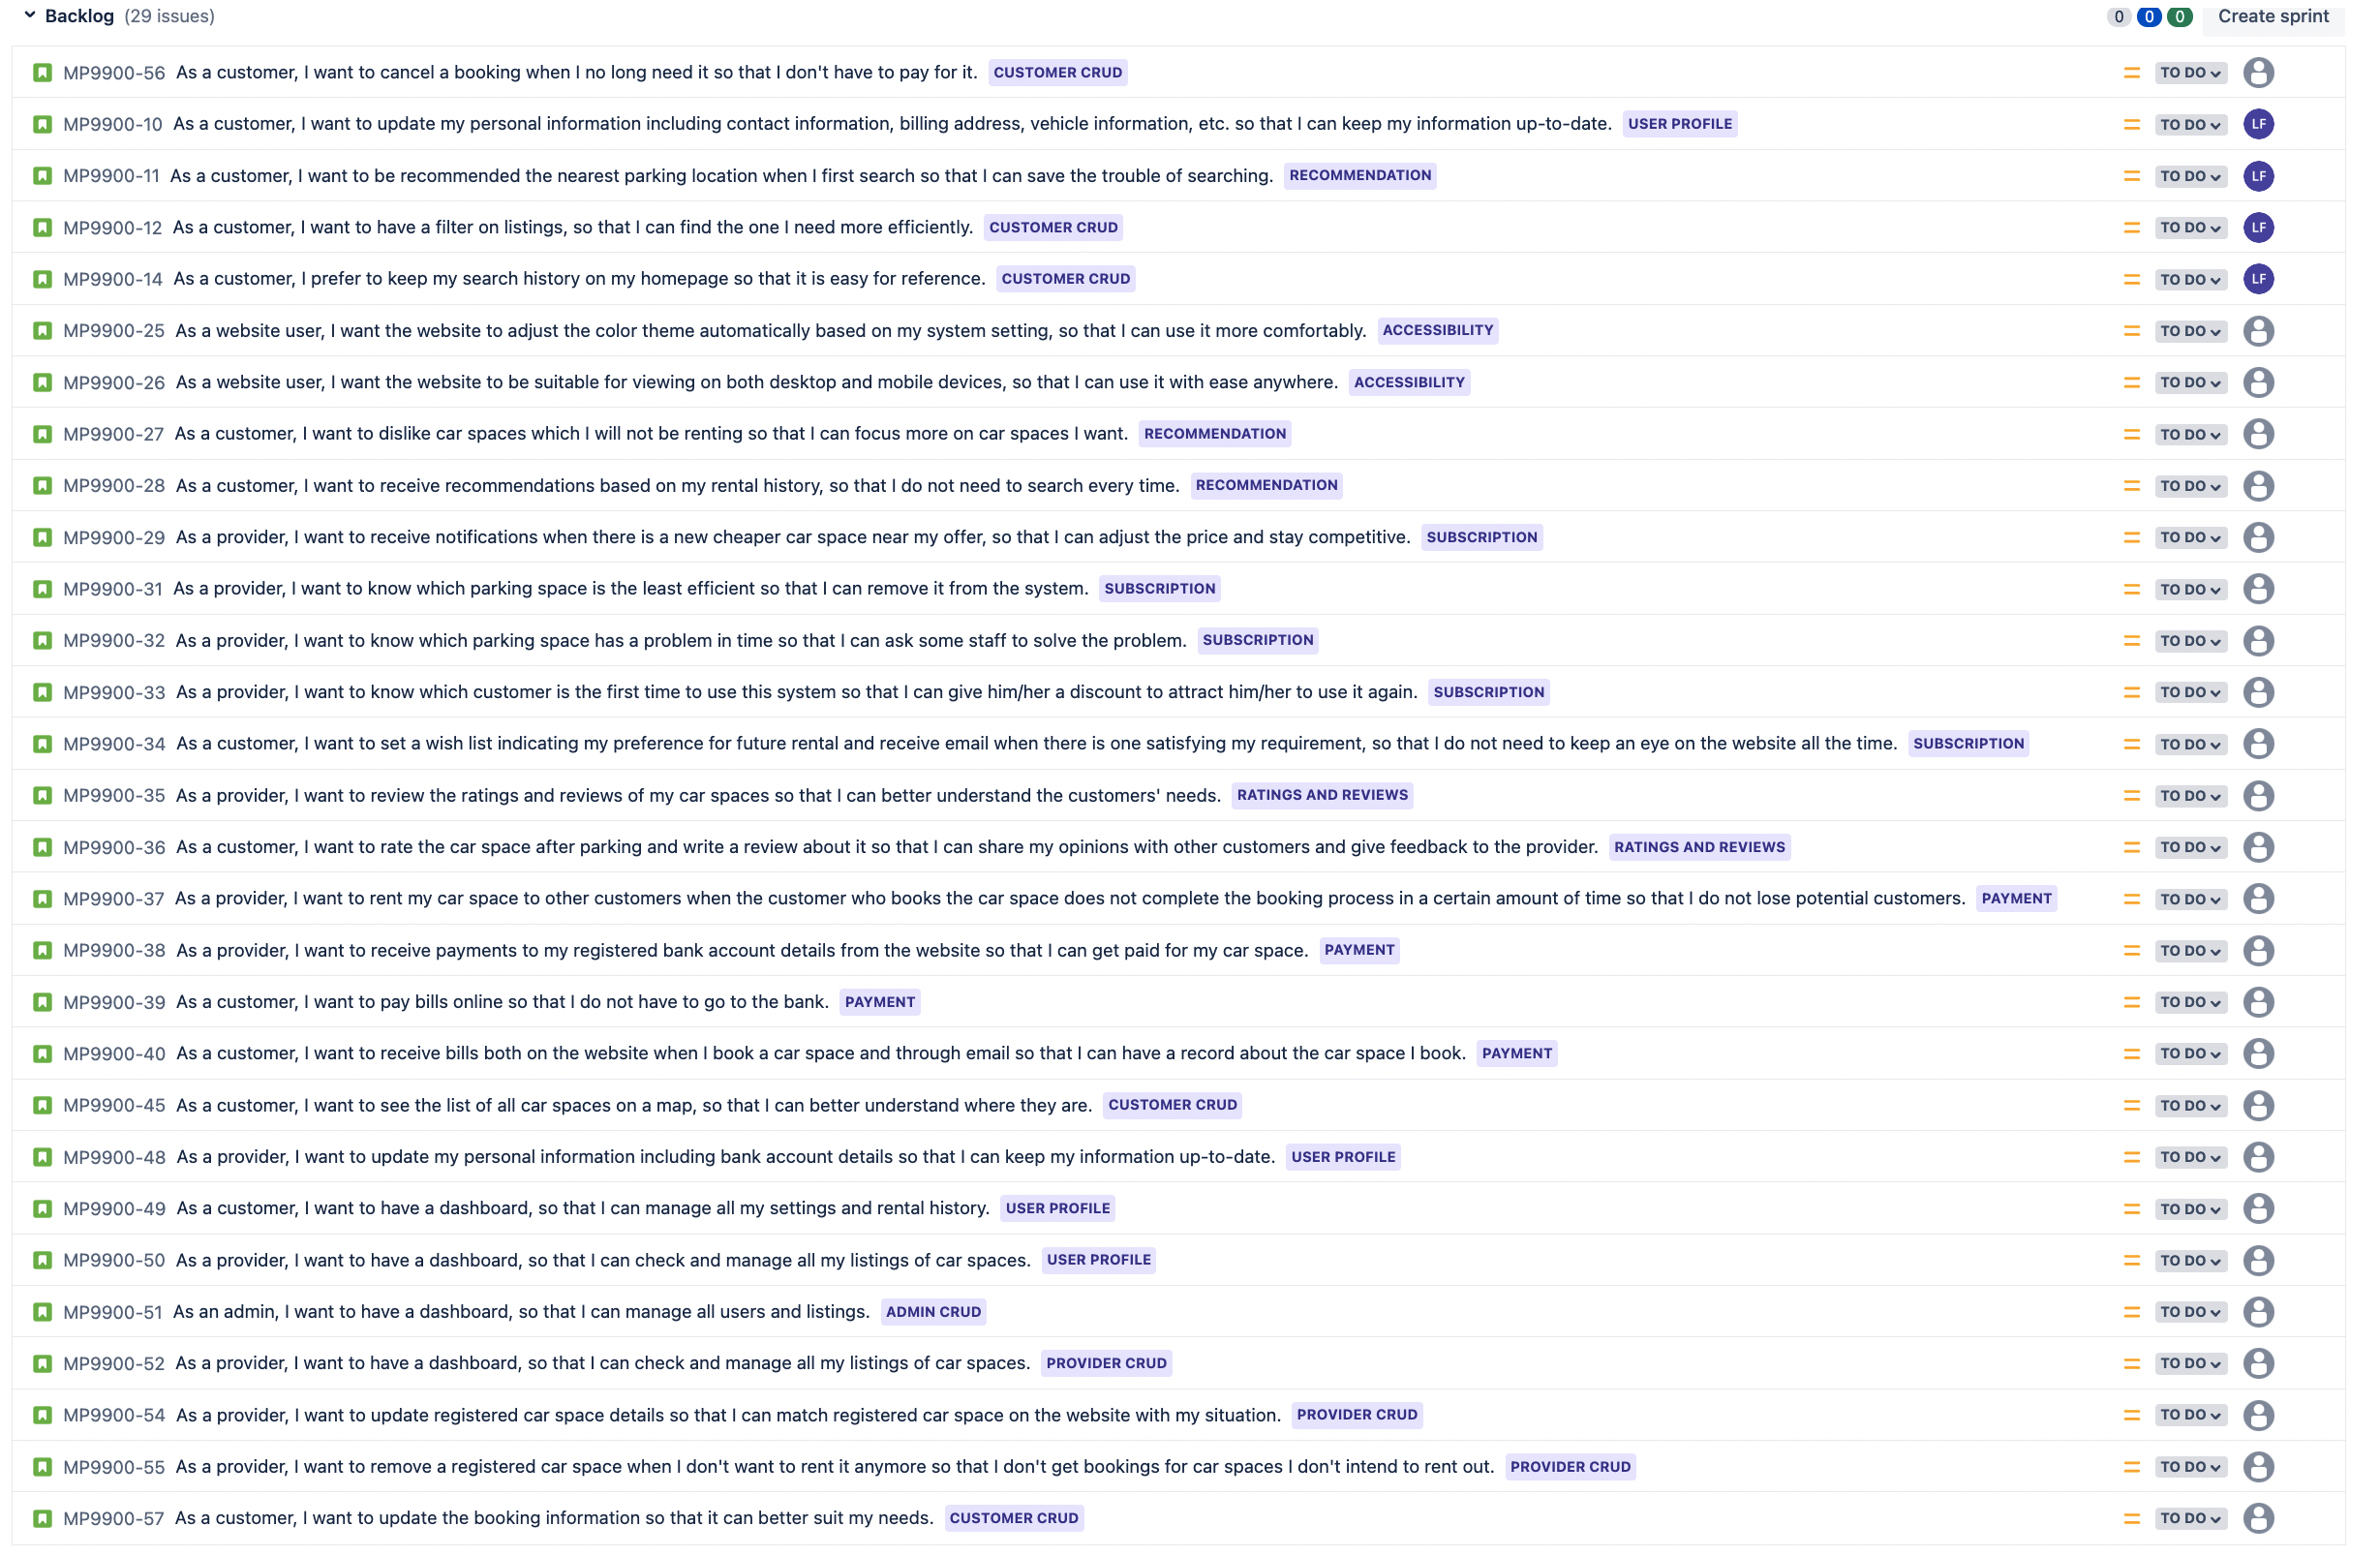
\includegraphics[width=\textwidth]{backlog.png}
  \caption{Backlog from Jira}
  \end{figure}

\section{Interface and Flow Diagrams}
  \subsection{Interface Design}
  \begin{figure}[htp]
    \centering
    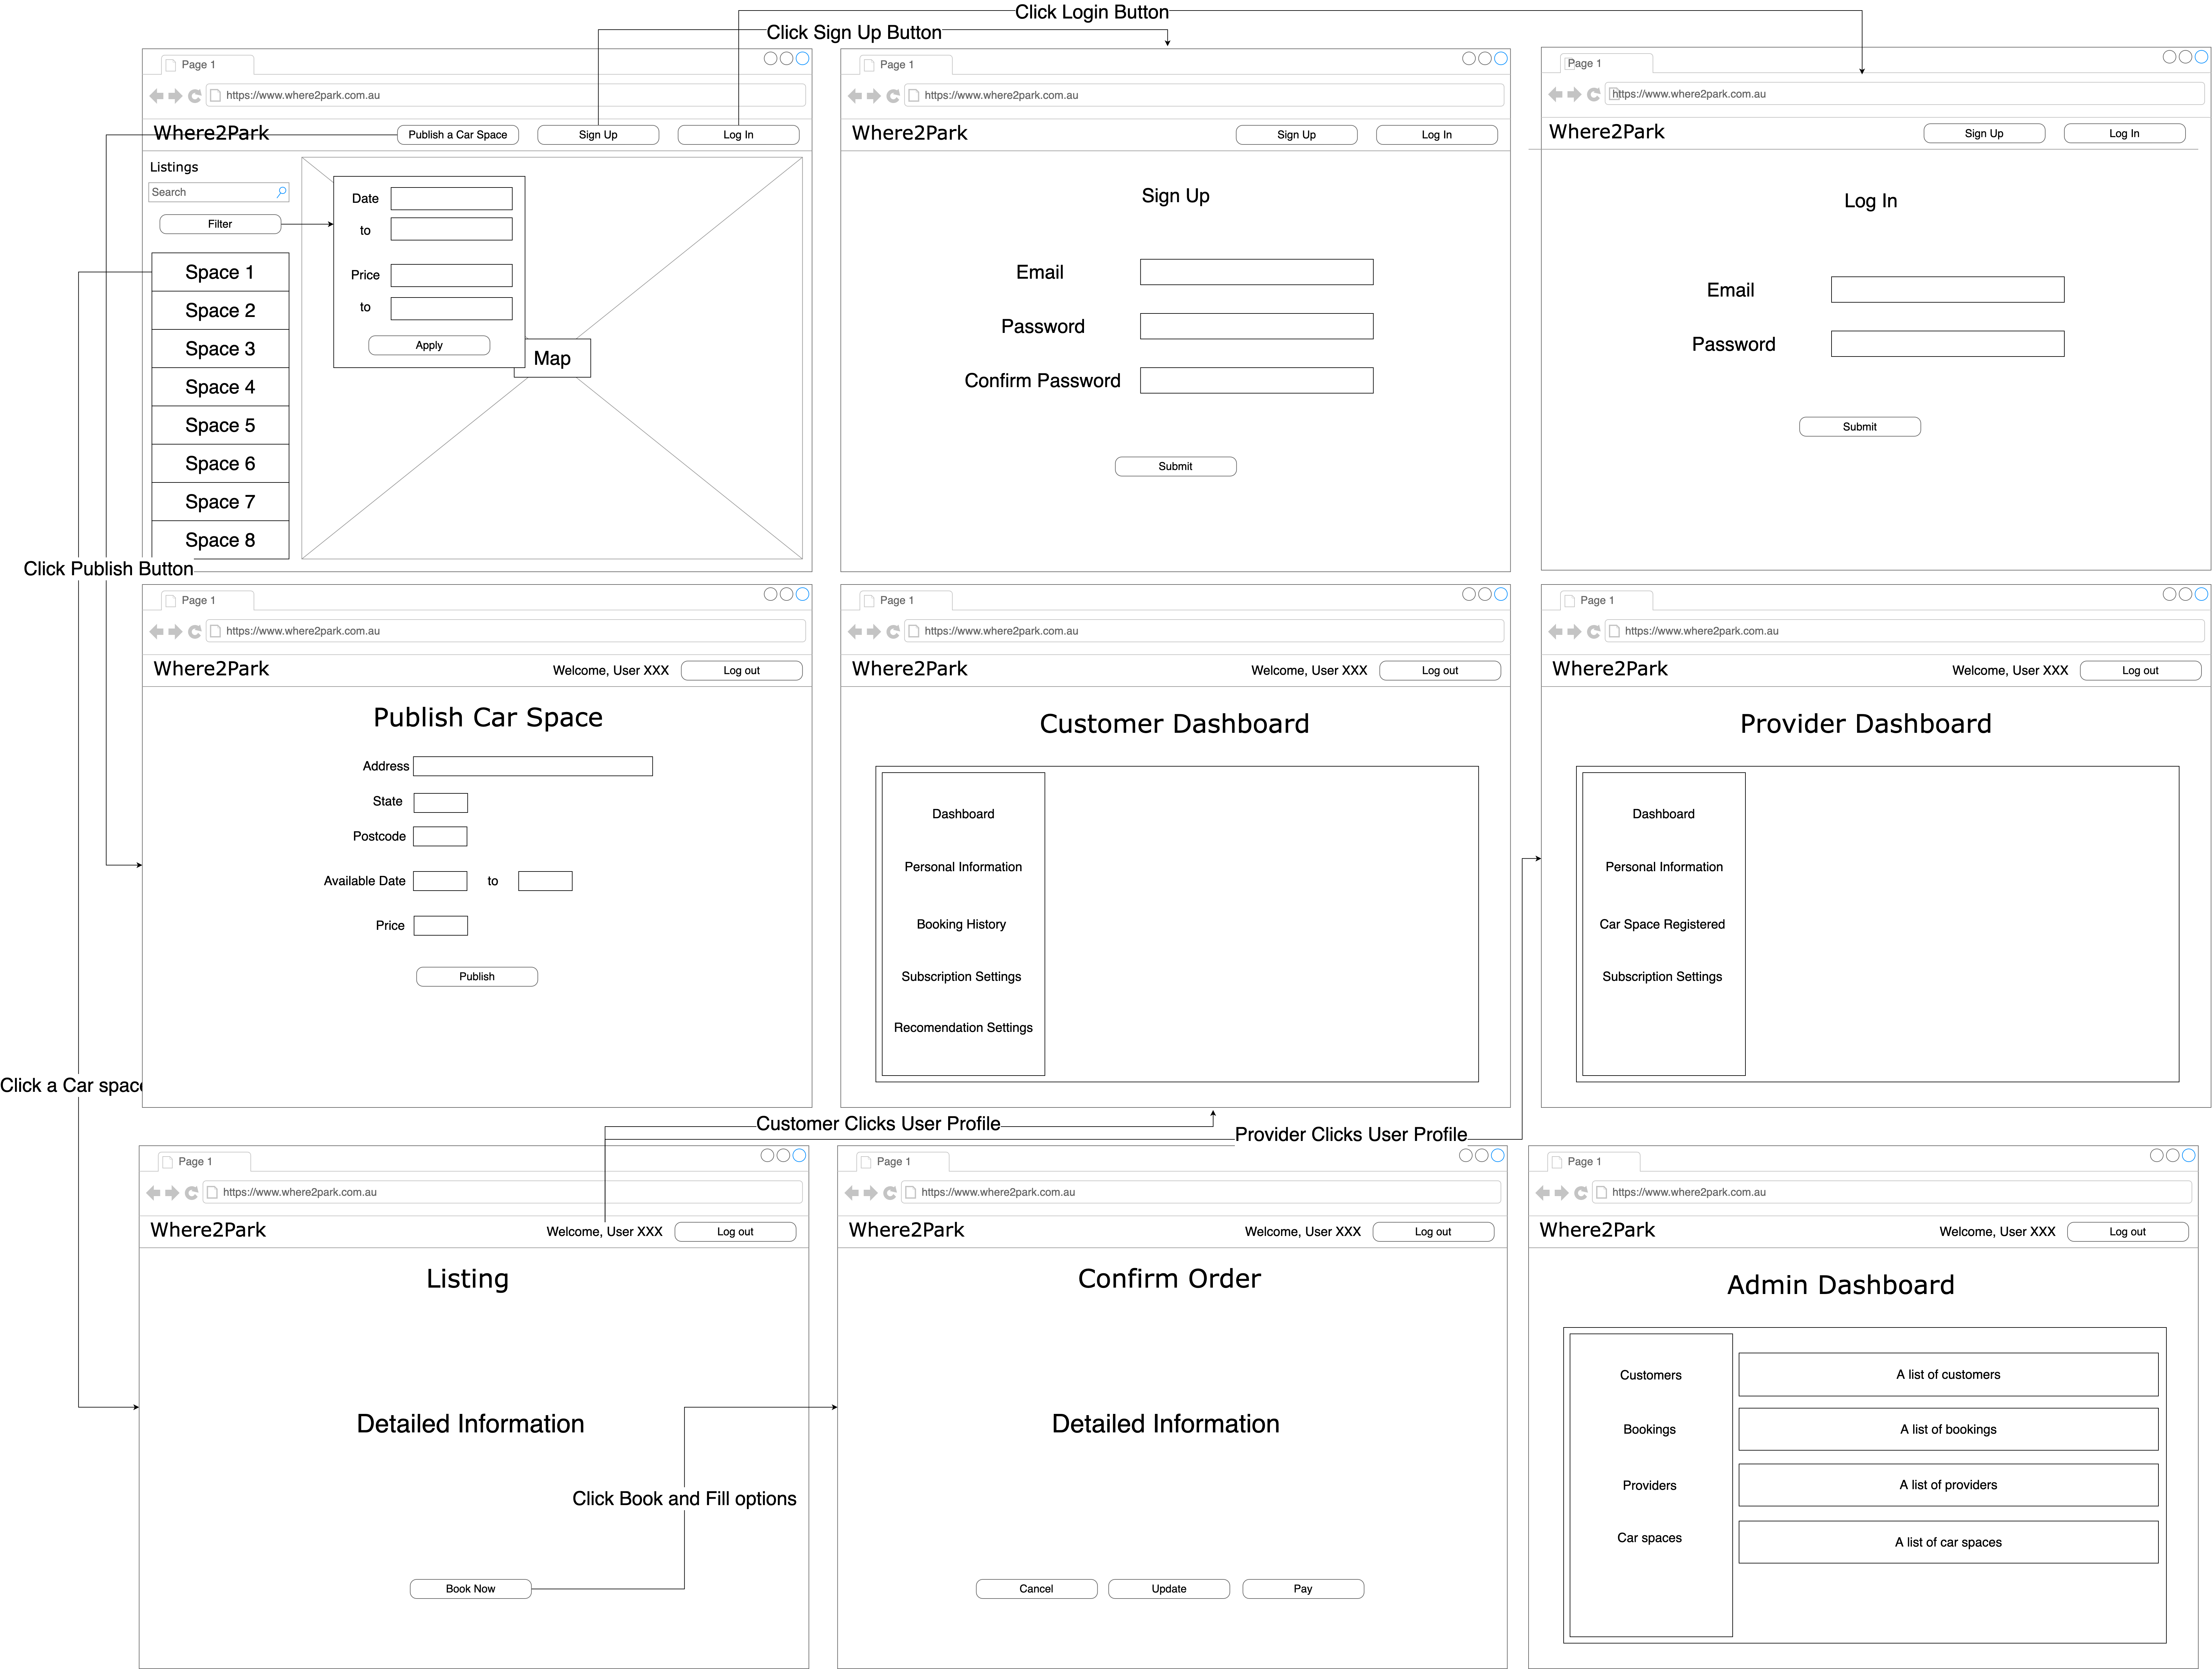
\includegraphics[width=\textwidth]{UI Design-UI.drawio.png}

  \caption{UI Design}
  \end{figure}
  \newpage
  \subsection{Flow Chart}

    \begin{figure}[htp]
      \centering
    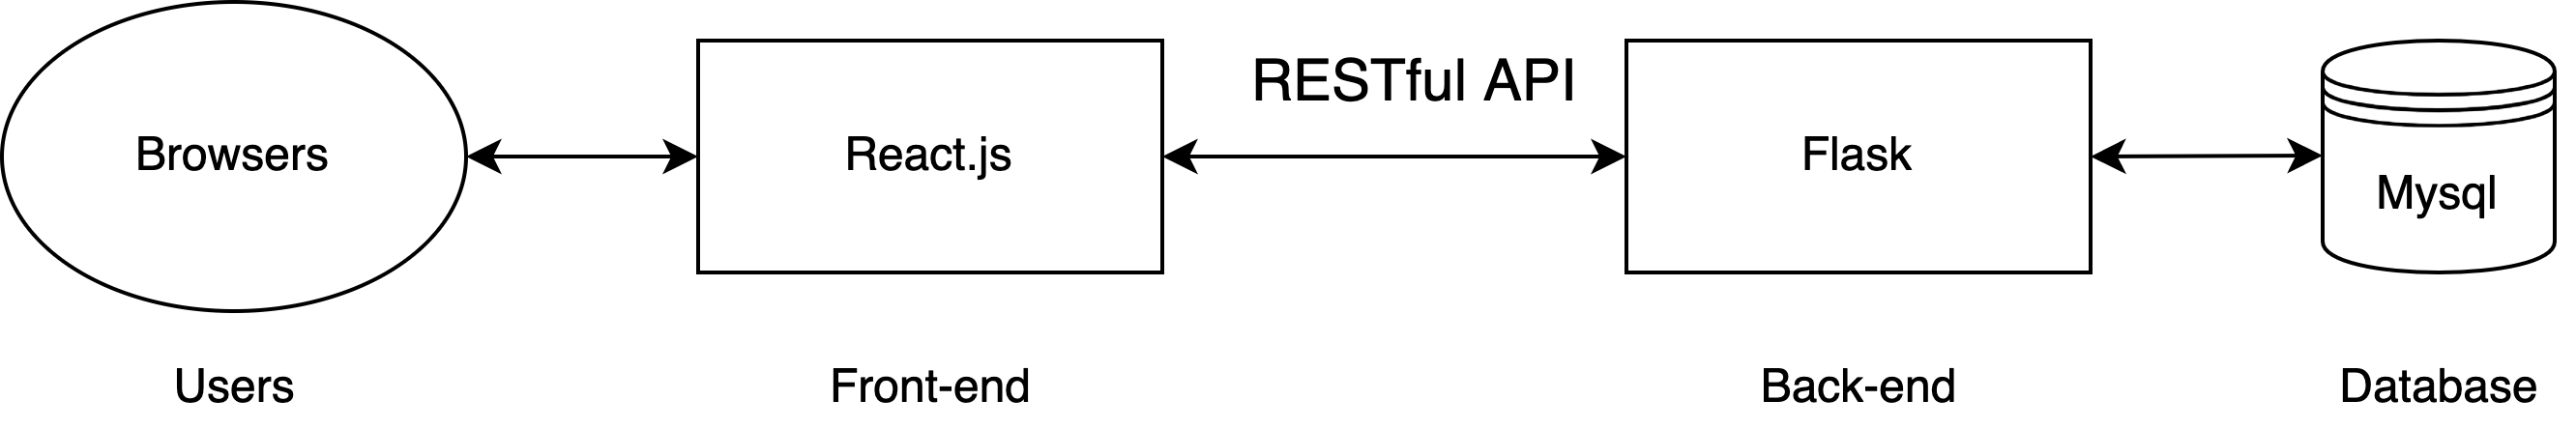
\includegraphics[width=0.9\textwidth]{UI Design-System Architecture.drawio.png}
    
    \caption{System Architecture}
    \end{figure}

  \subsection{Database Model}
  \begin{figure}[htp]
    \centering
  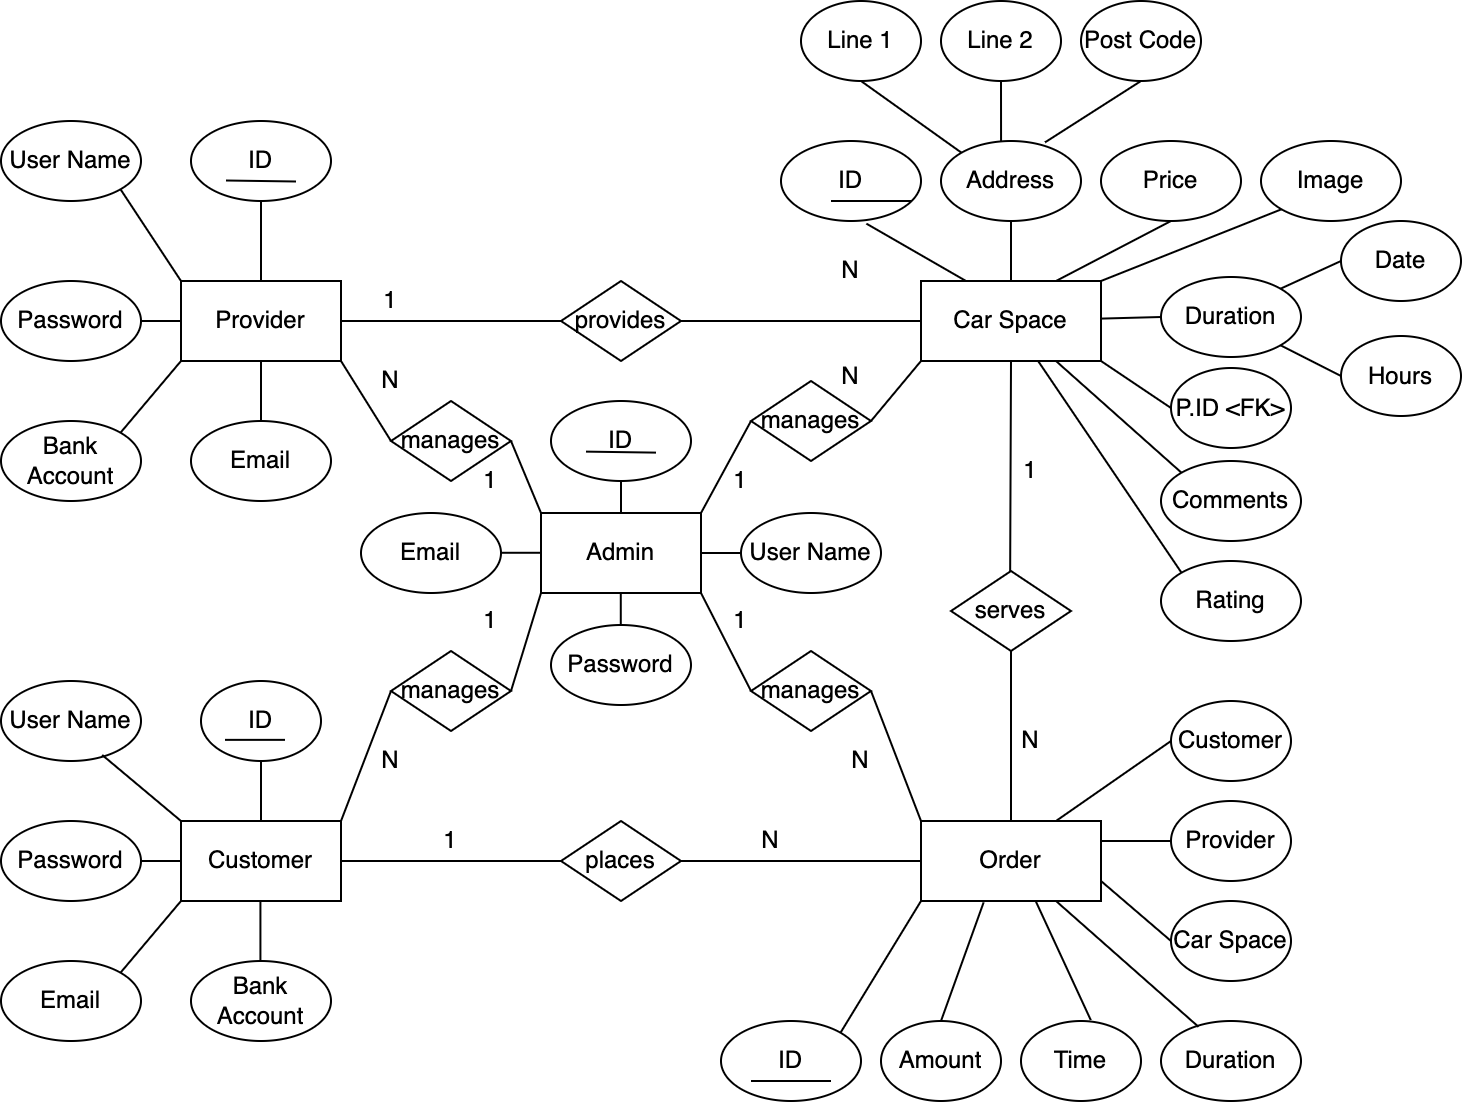
\includegraphics[width=0.9\textwidth]{UI Design-ER.drawio.png}
  
  \caption{System Architecture}
  \end{figure}
  \subsection{Page Definitions}
  
  Base on the functionalities, we should have following main pages:

  \begin{enumerate}
    \item
    \begin{description}
      \item[Home Page]
    \end{description}
    
    The first page users see when entering the website. With all listings and a map.

      \begin{enumerate}
        \item
        \begin{description}
          \item[Before Login]
        \end{description}

        The page has login and sign up buttons.

        \item     
        \begin{description}
          \item[After Login]
        \end{description}

        The page contains user information, e.g. the avatar or username and provides a button to log out.
      \end{enumerate}

    \item
    \begin{description}
      \item[Login Page]
    \end{description}

    The page contains a form for logging in.
  
    \item
    \begin{description}
      \item[Sign Up Page]
    \end{description}
  
    The page contains a form for signing up.

    \item
    \begin{description}
      \item[Car Space Detail Page]
    \end{description}
  
    The page contains detailed information about the car space, e.g. location, availability, and reviews and allows customers to create a new booking.
  
    \item
    \begin{description}
      \item[Car Space Booking Preview Page]
    \end{description}

    The page displays the booking information in addition to the car space details, e.g. duration, and price.

      \begin{enumerate}
        \item
        \begin{description}
          \item[Before Payment]
        \end{description}
  
        The page has a button to pay for the booking and complete the order.
  
        \item     
        \begin{description}
          \item[After Payment]
        \end{description}
  
        The page contains confirmation of the payment.
  
      \end{enumerate}

    \item
    \begin{description}
      \item[Provider profile Page]
    \end{description}

      \begin{enumerate}
        \item
        \begin{description}
          \item[Dashboard]
        \end{description}
    
        The page contains statistics about registered car spaces.
    
        \item     
        \begin{description}
          \item[Personal Information]
        \end{description}

        The page contains personal information and allows change including banking information.
    
        \item     
        \begin{description}
          \item[Car Space Registered]
        \end{description}

        The page contains a registered car space list.

        \item     
        \begin{description}
          \item[Subscription Settings]
        \end{description}

        The page allows the provider to choose from multiple subscription settings.       

      \end{enumerate}

      \begin{figure}[htp]
        \centering
      \includegraphics[width=0.9\textwidth]{UI Design-Provider Profile Page.drawio.png}
      
      \caption{Provider Profile Page UI}
      \end{figure}

      \item
      \begin{description}
        \item[Customer Profile Page]
      \end{description}
    
      The page contains customer information and allows customers to update it.
  
        \begin{enumerate}
          \item
          \begin{description}
            \item[Dashboard]
          \end{description}
      
          The page contains statistics about booking history.
      
          \item     
          \begin{description}
            \item[Personal Information]
          \end{description}
  
          The page contains personal information and allows change, including banking information.
  
          \item     
          \begin{description}
            \item[Booking History]
          \end{description}
  
          The page contains a list of bookings made.
  
          \begin{enumerate}
            \item         
            \begin{description}
              \item[Current Booking]
            \end{description}
  
            The page contains current unpaid bookings and allows the customer to update, cancel or complete them.
  
            \item         
            \begin{description}
              \item[Old Booking]
            \end{description}
  
            The page contains previous bookings.
  
          \end{enumerate}
  
          \item     
          \begin{description}
            \item[Subscription Settings]
          \end{description}
  
          The page allows the customer to choose from multiple subscription settings.       
  
  
          \item     
          \begin{description}
            \item[Recommendation Settings]
          \end{description}
  
          The page allows the customer to choose from multiple recommendation settings.    
  
        \end{enumerate}
  
        \begin{figure}[htp]
          \centering
        \includegraphics[width=0.9\textwidth]{UI Design-Customer Profile Page.drawio.png}
        
        \caption{Customer Profile Page UI}
        \end{figure}

      \item
      \begin{description}
        \item[Register a new car space Page]
      \end{description}

      The page contains a form, allowing the provider to register a new car space.

      \item
      \begin{description}
        \item[Admin Dashboard]
      \end{description}

      The page contains data about customers, providers, car spaces and bookings.

  \end{enumerate}

\textit{Note: The above-mentioned pages are a representation of the main functions of the system. It is by no means a comprehensive list, and it is possible to differ from the end result.}

\section{System Architecture}

  We adopt the method of the separation of front-end and backend and use Rest API to connect both. As team members have different skills and experiences in application development, we believe this way can reach fast development and each member has less content to think about.

  \subsection{Front-end}
  
  For the front-end application, we choose Next.js as the development framework.

  With all these years of evolution in front-end development, front-end engineers no longer need to write plain JavaScript for web applications. Thanks to React and other frameworks, we can write more powerful applications in less time. Since React is one of the most popular frameworks in the market, we choose it to be the framework for the front-end of our application.
  
  On top of that, Next.js integrates all the features we need for production, and it provides an excellent development experience as well. We will be using a script provided by Next.js to start our front-end application.
  
  \subsection{Backend}
  
  For the backend application, we choose Flask as the development framework.

  Flask is chosen because it is a lightweight framework and is relatively simple, which is coupled with the presence of jinja2 modules in Flask, making the cost of learning cheaper for less experienced members.
  
  The main language chosen for the back terminal system is Python. Python is a popular programming language and its community is very active, resulting in a large number of third-party libraries and modules. Also, team members have had experience in Python.
  
  \subsection{Authorization}
  
  The authorization process guarding all interactions between users and the application is 
  \href{https://jwt.io/introduction}{JSON Web Tokens}.
  
  The detailed authorization process is shown below.
  

  \begin{figure}[htp]
    \centering
  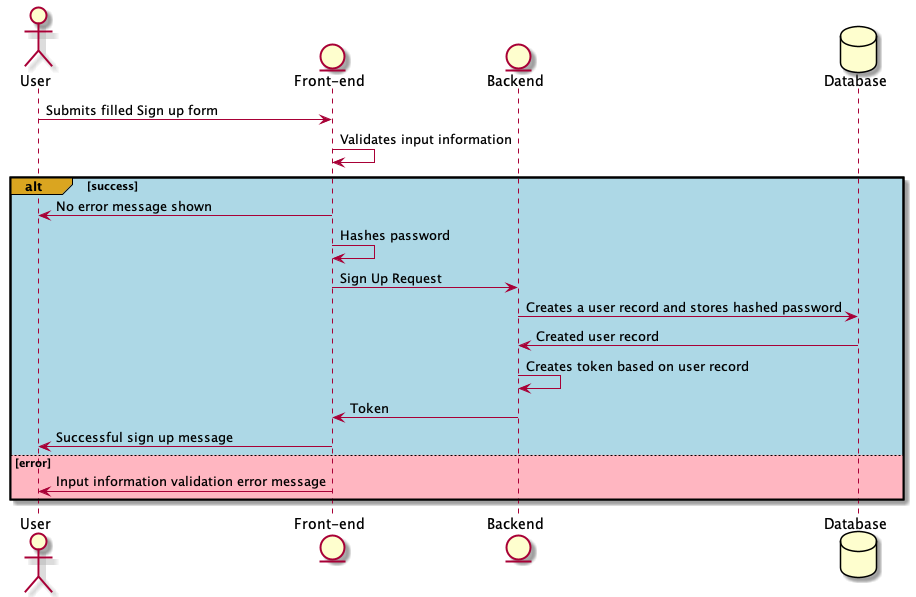
\includegraphics[width=0.9\textwidth]{Sign Up Sequence Diagram.png}
  
  \caption{Sign Up Sequence Diagram}
  \end{figure}

  \begin{figure}[htp]
    \centering
  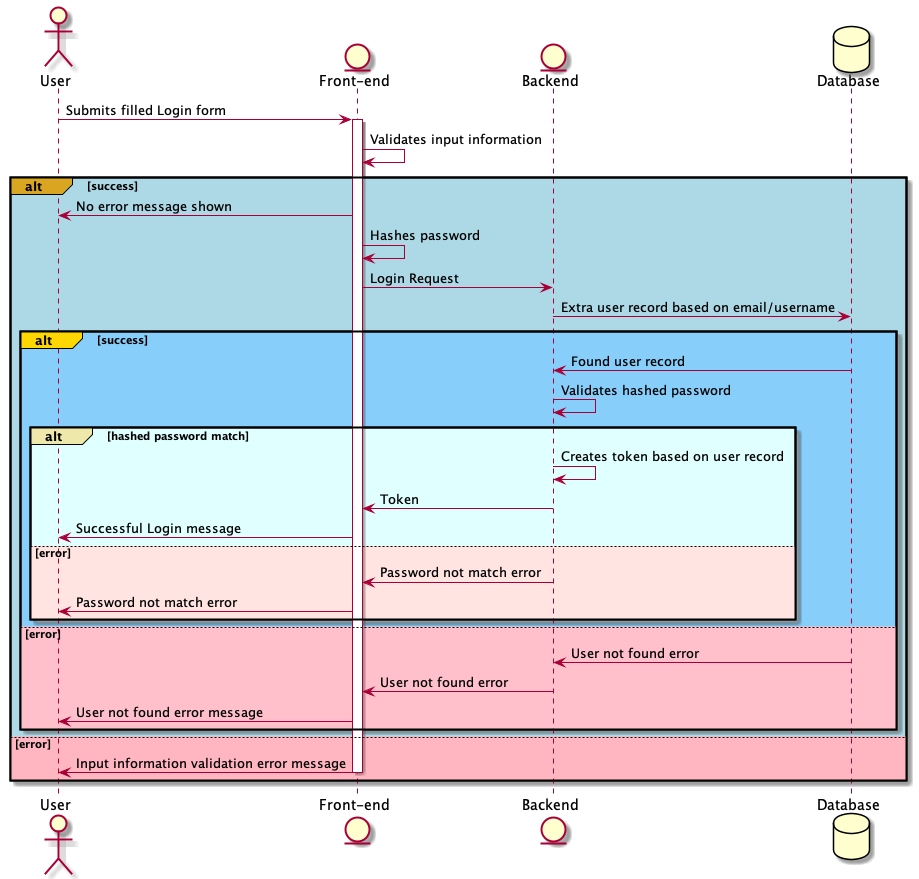
\includegraphics[width=0.9\textwidth]{Login Sequence Diagram.png}
  
  \caption{Login Sequence Diagram}
  \end{figure}


\begin{thebibliography}{9}
  \bibitem{covid-travel}
  Beck MJ, Hensher DA. Insights into the impact of COVID-19 on household travel and activities in Australia - The early days of easing restrictions. Transp Policy (Oxf). 2020 Dec;99:95-119. doi: 10.1016/j.tranpol.2020.08.004. Epub 2020 Aug 18. PMID: 32836998; PMCID: PMC7434414.
\end{thebibliography}
\end{document}